\chapter{Writing \LaTeX{}}\label{cha:c1_firstchapter}

This document shows how you can get ePub-like formatting in \LaTeX{} with the \verb|memoir| document class. You can't yet export directly to ePub from writeLaTeX, but you can download the source and run it through a format conversion tool, such as \verb|htlatex| to get HTML, and then go from HTML to ePub with a tool like Sigil or Calibre. See \url{http://tex.stackexchange.com/questions/16569} for more advice. And they lived happily ever after.

\section{Basic Formatting}\label{sec:c1_basicformatting}

\paragraph{Comments.} If you want to just add a comment to a file without it
being printed, add a \lstinline[language=Tex]!%! (percentage) sign in front of
it. In the template files, you will find a number of such
comments as well as deactivated commands.

\paragraph{Bold formatting.} You can make your text bold by surrounding it
with the command \lstinline[language=Tex]!\textbf{}!.

\paragraph{Italics formatting.} You can make your text italic by surrounding
it with the command \lstinline[language=Tex]!\textit{}!.

\paragraph{Small caps.} You can change your text into small capitals by
surrounding it with the command \lstinline[language=Tex]!\textsc{}!.
    
\paragraph{Text em dashes.} Em dashes are used to connect two related sentences.
There is no space before or after the em dash. Within the template, use the
command \lstinline[language=Tex]!\textemdash{}! instead of using the dash you
copied over from your text file. This will also take care of issues relating to
line breaks.

\paragraph{Paragraphs.} Paragraphs are handled automatically by leaving an empty
line between each paragraph. Adding more than one empty line will not change
anything\textemdash{}remember it is not a ``what you see is what you get''
editor.

\paragraph{Empty line.} If you want to force an empty line (recommended only in
special cases), you can use \lstinline[language=Tex]!~\\! (tilde followed by two
backslashes).

\paragraph{New page.} Pages are handled automatically by \LaTeX{}. It tries to
be smart in terms of positioning paragraphs and pictures. Sometimes it is
necessary to add a page break, though (ideally, at the very end when polishing
the final text). For that, simply add a \lstinline[language=Tex]!\newpage!.

\paragraph{Quotation marks.} In the normal computer character set, there are
more than one type of quotation marks. It is required to change all quotation
marks into \lstinline[language=Tex]!``\dots''! (two back ticks at the beginning
and two single ticks at the end) and refrain from using ``\dots'' (or “\dots”)
altogether. This is because Word's “\dots” uses special characters, and ``\dots'' do not mark the beginning and end of the quotation.

\paragraph{Horizontal line.} For a horizontal line, simply write \lstinline[language=Tex]!\toprule!, \lstinline[language=Tex]!\midrule!, or \lstinline[language=Tex]!\bottomrule! from booktabs. You can also use the less recommend \lstinline[language=Tex]!\hline!. % chktex 44

\paragraph{Underlined text.} It is generally not recommended to use underlined
text.

\paragraph{URLs.} For URLs you need a special monospaced font. Also, for URLs in
e-books, you want to make them clickable. Both can be accomplished by putting
the URL in the \lstinline[language=Tex]!\url{}! environment, for example
\lstinline[language=Tex]!\url{https://www.lode.de}!.

\paragraph{Special characters.} If you need special characters or mathematical
formulas, there is a whole body of work on that subject. It is not in the scope
of this book to provide you a comprehensive list.

\section{Lists}\label{sec:c1_lists}

\paragraph{Itemized list.} To create a bullet point list (like the list in this
section), use the following construct:%
\begin{lstlisting}[language=Tex]
\begin{itemize}
    \item Your first item.
    \item Your second item.
    \item Your third item.
%   \item Your commented item.
\end{itemize}
\end{lstlisting}

The result will look like this:%
\begin{itemize}
    \item Your first item.
    \item Your second item.
    \item Your third item.
% 	\item Your commented item.
\end{itemize}

\paragraph{Numbered list.} To create a numbered list, replace itemize with
enumerate:%
\begin{lstlisting}[language=Tex]
\begin{enumerate}
    \item Your first item.
    \item Your second item.
    \item Your third item.
\end{enumerate}
\end{lstlisting}

The result will look like this:%
\begin{enumerate}
	\item Your first item.
	\item Your second item.
	\item Your third item.
\end{enumerate}


\section{Verbatim text}\label{sec:c1_verbatim}

Sometimes, you do want to simply use text in a verbatim way (including special
characters and \LaTeX{} commands). For this, simply use the
\lstinline[language=Tex]!\lstlisting! environment:
\lstinline[language=Tex]!\begin{lstlisting}...\end{lstlisting}!%
. For example, I put the itemize and enumerate listings above into a
\lstinline[language=Tex]!\lstlisting! block. If I did not, \LaTeX{} would have
displayed the list as a list, instead of displaying the code.



\section{Chapters and Sections}\label{sec:c1_chaptersandsections}

\LaTeX{} uses a hierarchy of chapters, sections, and subsections. There are also
sub-subsections, but for the sake of the reader, it is best to not go that deep.
If you come across a situation where it looks like you need it anyway, I
recommend thinking over the structure of your book rather than using
sub-subsections. 

In terms of their use in the code, they are all similar:

\begin{itemize}
    \item \lstinline[language=Tex]!\chapter{Title of the Chapter}\label{cha:c1_chaptername}!
    \item \lstinline[language=Tex]!\section{Title of the Section}\label{sec:c1_sectionname}!
    \item \lstinline[language=Tex]!\subsection{Title of the Subsection}\label{subsec:c1_subsectionname}!
    \item \lstinline[language=Tex]!\paragraph{Title of the Paragraph}\label{par:c1_paragraph}!
\end{itemize}

When using these commands, obviously replace the title, but also the label. For
the label, I recommend to have it start with either ``cha:'', ``sec:'', ``subsec:'', etc.\ to specify what kind of label it is, followed with c and the current chapter number, an underscore, and the chapter, section, or subsection in one word and lowercase. These labels can then be used for references like we used previously for the images. For example, if you have defined a section
\lstinline[language=Tex]!\section{Chapters and Sections}\label{sec:c1_chaptersandsections}!, 
you could write ``We will discuss chapters
and sections in section
\lstinline[language=Tex]!\cref{sec:c1_chaptersandsections}!'' which results in the document in ``We will discuss chapters and sections in \cref{sec:c1_chaptersandsections}''.


\section{Tables}\label{sec:c1_tables}

In \LaTeX{}, tables are like images and put into the figure environment. As
such, they have a caption, label, and a positioning like we discussed above with
the images. Drawing a table requires a bit of coding:
\begin{lstlisting}[language=Tex]
\begin{table}[!ht]
    \centering
    \begin{tabular}{p{2.5cm}|p{3.5cm}|p{3.5cm}}
    \hline
    & \textbf{Word} & \textbf{\LaTeX{}} \\ 
    \hline
    
    Editor & ``what you see is what you get'' & source file is compiled \\
    \hline
    
    Compatibility & dependent on editor & independent of editor \\
    \hline
    
    Graphics & simple inbuilt editor & powerful but complex editor \\
    \hline
    
    Typography & optimized for speed & optimized for quality \\
    \hline
    
    Style & inbuilt style & separate style document \\
    \hline
    
    Multi-platform & only via export & possible with scripting \\
    \hline
    
    Refresh & some elements need, manual refresh & everything is refreshed with each compile \\
    \hline
    
    Formulas & basic support needs external tools & complete support \\
    \hline
    
    \end{tabular}
    \caption{Comparison of Word and \LaTeX{}} \label{tab:c1_comparisonwordlatex}
\end{table}
\end{lstlisting}

This table from the beginning of the book has the familiar figure, label,
caption, and centering commands. The actual table is configured with the
\lstinline[language=Tex]!\tabular{}! environment. Following the tabular command,
you configure the columns in curly braces. Each column is separated with a
vertical line and the \lstinline[language=Tex]!p{...}! % chktex 11
entry specifies the width
of the column. With \lstinline[language=Tex]!{p{2.5cm}|p{3.5cm}|p{3.5cm}}!, you
would have three columns with 2.5cm width for the first column and 3.5cm width
for the two others. Alternatively, you can use \lstinline[language=Tex]!c!
instead of \lstinline[language=Tex]!p! and leave out the curly braces with the
width. Then, \LaTeX{} simply calculates the required widths automatically. Then,
for each line of the table, simply write: 
\lstinline[language=Tex]!content of the first cell & content of the second cell & content of the third cell\\\midrule!.

\begin{table}[!ht]
    \centering
    \begin{tabular}{p{2.5cm}p{3.5cm}p{3.5cm}}
        \toprule
        & \textbf{Word} & \textbf{\LaTeX{}} \\ 
        \midrule
        
        Editor & ``what you see is what you get'' & source file is compiled \\
        \midrule
        
        Compatibility & dependent on editor & independent of editor \\
        \midrule
        
        Graphics & simple inbuilt editor & powerful but complex editor \\
        \midrule
        
        Typography & optimized for speed & optimized for quality \\
        \midrule
        
        Style & inbuilt style & separate style document \\
        \midrule
        
        Multi-platform & only via export & possible with scripting \\
        \midrule
        
        Refresh & some elements need, manual refresh & everything is refreshed with each compile \\
        \midrule
        
        Formulas & basic support needs external tools & complete support \\
        \bottomrule
    
    \end{tabular}
    \caption{Comparison of Word and \LaTeX{}}\label{tab:c1_comparisonwordlatex}
\end{table}

\section{Footnotes}\label{sec:c1_footnotes}

Finally, for footnotes, there is the command
\lstinline[language=Tex]!\footnote{}!. You can place it anywhere you like,
\LaTeX{} will then automatically add the number of the footnote at that place,
and put the footnote text into the footer area. It looks like
this.\footnote{This is a footnote.} The challenge here relates to grammar:
footnotes start with capital letters, parentheses with lower case, and the
footnote comes after the period, the parentheses have to start before the
period.

\section{Inserting Images}\label{sec:c1_images}

As in Word, in \LaTeX{}, images are separate from the text. Images are usually
packaged together with a caption and a label to reference it from the text.
These three entities are packaged together into a figure. The figure itself
configures the size of the image as well as where it should be put. Let us look
at a code sample:
\begin{lstlisting}[language=Tex]
\begin{figure}[!ht]
    \centering
    \includegraphics{images/ebookLatex_Cover.jpg}
    \caption{The cover of this book.} \label{fig:c1_cover}
\end{figure}
\end{lstlisting}

Let us go through this line by line. At the core is the image, included with
\lstinline[language=Tex]!\includegraphics{path to file}!. It inserts the image
specified by the ``path to file.'' With the
\lstinline[language=Tex]!\adjustbox{}! command, we can adjust the image size
according to the page width (\lstinline[language=Tex]!\columnwidth!) and page
height (\lstinline[language=Tex]!\textheight!). 

Below there is the caption and the label. \LaTeX{} automatically numbers each
figure, so in the text, we can later refer to it with
\lstinline[language=Tex]!\ref{c1_cover:fig}! which prints out the number of the
figure. Finally, all these commands are centered with the
\lstinline[language=Tex]!\centering! command and surrounded with the figure
environment. The \lstinline[language=Tex]![!ht]! instructs \LaTeX{} to try to
place the image exactly where it is in the \LaTeX{} code.

\begin{figure}[!ht]
	\centering
	
\includegraphics{images/cover.jpg}
	\caption{The cover of this book.}\label{fig:c1_cover}
\end{figure}

In \Cref{fig:c1_cover}, you can see the result of the command. Instead of
graphics, you can also include other TEX files that contain graphics (or
commands to draw graphics, see \Cref{sec:c1_tikzgraphics}).

\section{TikZ Graphics}\label{sec:c1_tikzgraphics}

For graphics, you can use the inbuilt TikZ graphics generator. Due to its
flexibility, I even recommend images you already have for a number of reasons:

\begin{itemize}
    \item TikZ graphics can very easily changed (especially for for example
    translations or making corrections).
    \item TikZ graphics are small and flexible. They can be easily scaled to any
    size and are directly integrated into your project (no time-consuming
    editing in an external graphics program necessary).
    \item TikZ graphics look better. As vector graphics are sent directly to the
    printer, we need not to worry about readability.
\end{itemize}

If you want to create a TikZ graphic, simply create a new TEX file in the
\textit{tex-images} folder and include it with \lstinline[language=Tex]!\input{...}! % chktex 27
(replacing \lstinline[language=Tex]!\includegraphics{}!) where you want to. 

Then, do a ``recompile from scratch'' by clicking on the top right corner of the
preview window (showing Warning or Error) to regenerate the TikZ file. If
``up-to-date and saved'' is shown, delete the \textit{tikz-cache} directory and
recreate it. 

For the format of the file itself, it is a series of commands surrounded by the
\lstinline[language=Tex]!\begin{tikzpicture}...\end{tikzpicture}!%
environment. Discussing all the commands is beyond the scope of this book, so I recommend three options:

\begin{itemize}
    \item Check out the PGF manual at \url{https://www.ctan.org/pkg/pgf}. It is
    more than 1100 pages full with documentation of each command and
    corresponding examples.
    \item Check out the few example TikZ pictures from my two books~\cite{PFH1E, PFH2E} in the \textit{tex-images} directory.
\end{itemize}

\begin{figure}[!ht]
    \centering
    \begin{tikzpicture}
        \node[fill=yellow!80,ellipse] (origin) {Origin};
        \node[fill=blue!30,ellipse] (destination) at (15em,0) {Destination};
        \path (origin) edge[->] node[above,font=\footnotesize] {the journey}
        (destination);
    \end{tikzpicture}
    \caption{TikZ drawings will be output as SVG, which should be rendered by most modern browsers.}
\end{figure}

\begin{figure}[!ht]
    \centering
    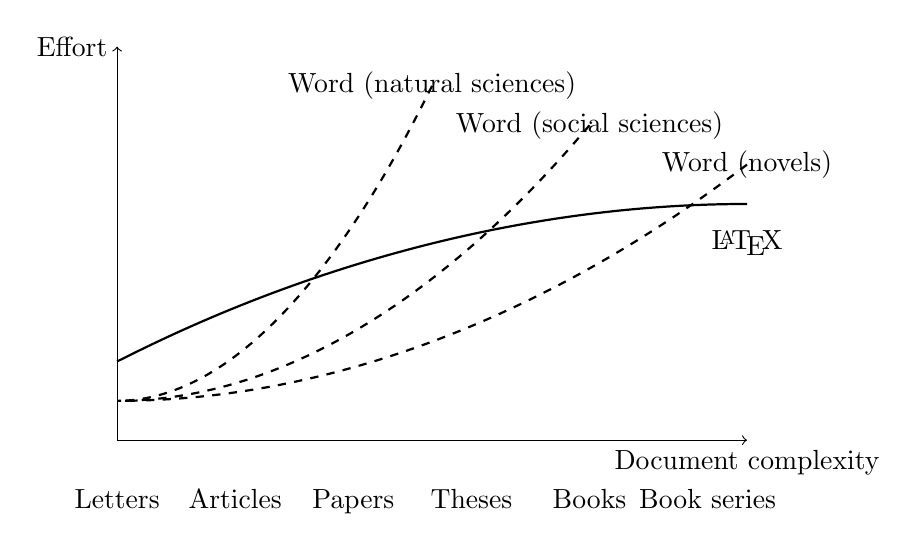
\begin{tikzpicture}

    % horizontal axis
    \draw[->] (0,0) -- (8,0) node[anchor=north] {Document complexity};
    \draw[->] (0,0) -- (0,5) node[anchor=east] {Effort};
    
    % labels
    \draw	(0,-0.5) node[anchor=north] {Letters}
    		(1.5,-0.5) node[anchor=north] {Articles}
    		(3,-0.5) node[anchor=north] {Papers}
    		(4.5,-0.5) node[anchor=north] {Theses}
    		(6,-0.5) node[anchor=north] {Books}
    		(7.5,-0.5) node[anchor=north] {Book series};
    
    \draw (8,3.5) node {Word (novels)};
    \draw (6,4) node {Word (social sciences)};
    \draw (4,4.5) node {Word (natural sciences)};
    \draw (8,2.5) node {\LaTeX{}};
    
    % Psis
    \draw[thick,dashed] (8,3.5) parabola[bend at end] (0,0.5);
    \draw[thick,dashed] (6,4) parabola[bend at end] (0,0.5);
    \draw[thick,dashed] (4,4.5) parabola[bend at end] (0,0.5);
    \draw[thick] (0,1) parabola[bend at end] (8,3);

\end{tikzpicture}
    \caption{Comparing complexity of \textit{Word} and \LaTeX{} depending on the application.}\label{fig:latexeffortcomplexity}
\end{figure}

\begin{figure}[!ht]
    \centering
    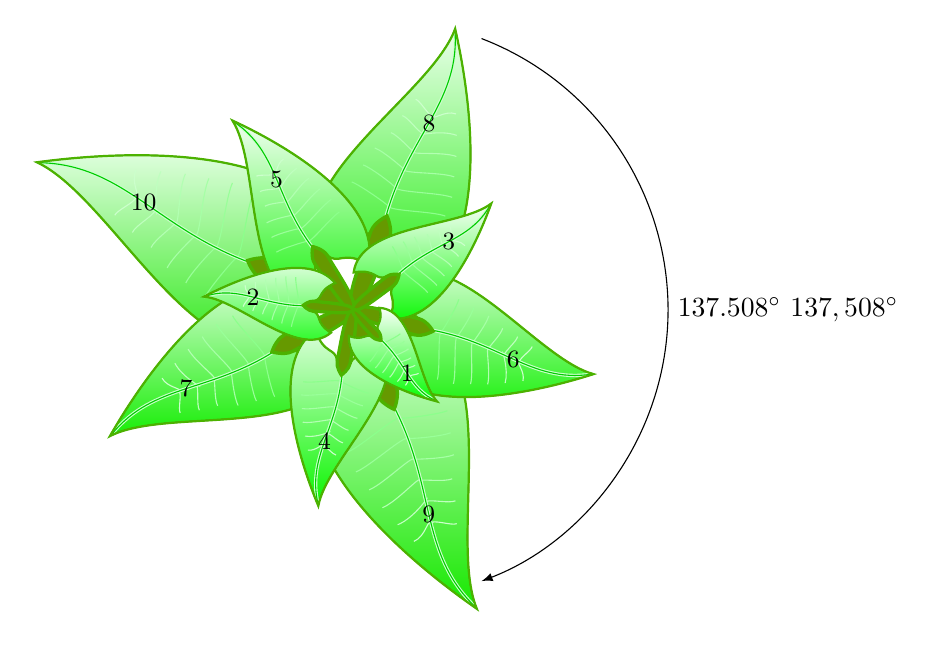
\begin{tikzpicture}
    \foreach \x in {10,...,1}
    {\draw[shade,bottom color=red!\x!green,top color=green!\x,x=0.3 pt,y=0.3 pt,scale={0.4+0.1*\x},rotate=222.5*\x] (0,0) .. 
    controls ( -11,  1) and ( -9, 50) .. (-10,80) ..
    controls ( -16, 60) and (-32, 75) .. (-50,40) .. 
    controls (-110,100) and (-0,230) ..  (  0,300)  node[below] (\x) {} ..
    controls (  45,230) and (110,100) .. ( 50,40) ..
    controls (  32, 75) and ( 16, 60) ..  ( 10,80) ..
    controls (   9, 50) and ( 11,  1) .. (  0,0) 
    -- cycle ;
    
    \draw[thin,green!45,x=0.3 pt,y=0.3 pt,scale={0.4+0.1*\x},rotate=222.5*\x] (-45,120) .. controls (-35,120) and (0,110) .. (-3,110) .. controls (0,105) and (40,120) .. (55,120);
    \draw[thin,green!40,x=0.3 pt,y=0.3 pt,scale={0.4+0.1*\x},rotate=222.5*\x] (-40,140) .. controls (-30,140) and (0,130) .. (-3,130) .. controls (0,125) and (40,140) .. (55,140);
    \draw[thin,green!35,x=0.3 pt,y=0.3 pt,scale={0.4+0.1*\x},rotate=222.5*\x] (-35,160) .. controls (-25,160) and (0,150) .. (0,150) .. controls (0,145) and (35,160) .. (50,160);
    \draw[thin,green!30,x=0.3 pt,y=0.3 pt,scale={0.4+0.1*\x},rotate=222.5*\x] (-25,180) .. controls (-17,180) and (0,170) .. (3,170) .. controls (0,165) and (30,180) .. (45,180);
    \draw[thin,green!25,x=0.3 pt,y=0.3 pt,scale={0.4+0.1*\x},rotate=222.5*\x] (-20,200) .. controls (-13,200) and (0,190) .. (6,190) .. controls (0,185) and (20,200) .. (38,200);
    \draw[thin,green!20,x=0.3 pt,y=0.3 pt,scale={0.4+0.1*\x},rotate=222.5*\x] (-13,220) .. controls (-8,220) and (3,210) .. (8,210) .. controls (10,205) and (18,220) .. (30,220);
    \draw[very thick,green!20,x=0.3 pt,y=0.3 pt,scale={0.4+0.1*\x},rotate=222.5*\x] (0,90) .. controls (-10,180) and (30,230) .. (1,297);
    \draw[thin,black!20!green,x=0.3 pt,y=0.3 pt,scale={0.4+0.1*\x},rotate=222.5*\x] (0,90)  .. controls (-10,180) and (30,230)  .. (1,297) node[midway,black] (num\x) {\small\x};
    \draw[very thick,red!30!green,fill=red!40!green,x=0.3 pt,y=0.3 pt,scale={0.4+0.1*\x},rotate=222.5*\x] 
    (0,0) .. 
    controls ( -11,  1) and ( -9, 50) ..
    (-10,80) .. 
    controls (-10,90) and (0,100) .. (0,100) ..
    controls (0,100) and (10,90) .. (10,80)..
    controls (   9, 50) and ( 11,  1) .. (  0,0) 
    -- cycle;
    \draw[thick,red!30!green,x=0.3 pt,y=0.3 pt,scale={0.4+0.1*\x},rotate=222.5*\x] (0,0) .. 
    controls ( -11,  1) and ( -9, 50) .. (-10,80) ..
    controls ( -16, 60) and (-32, 75) .. (-50,40) .. 
    controls (-110,100) and (-0,230) ..  (  0,300) ..
    controls (  45,230) and (110,100) .. ( 50,40) ..
    controls (  32, 75) and ( 16, 60) ..  ( 10,80) ..
    controls (   9, 50) and ( 11,  1) .. (  0,0) 
    -- cycle ;
    }
    \draw[->,>=latex,x=0.3 pt,y=0.3 pt,black] ([xshift=6pt] 8.east) arc (69:-69:350) node[midway,right] {$137.508^\circ$ $137,508^\circ$};
\end{tikzpicture}

    \caption{Example of a drawing made in TikZ.}\label{fig:leaves-golden-cut}
\end{figure}

\begin{figure}[!ht]
    \centering
    \begin{tikzpicture}
    % Define styles of various tikz elements.
    \tikzstyle{textbox} = [rounded corners, text width=60pt, minimum height=50pt,text centered,draw=black]
    \tikzstyle{arrow} = [thick,->,>=latex]
    \tikzstyle{block} = [rectangle,textbox]
    \tikzstyle{textarr} = [rectangle,align=center,fill=white]

    \node (latex) [block] {\LaTeX{}\\document};
    \node (overleaf) [block, left=of latex] {Overleaf};
    \node (pdf) [block, above left=of overleaf] {PDF}; % xelatex
    \node (html) [block, above right=of overleaf] {HTML}; % pdfLaTeX + tex4ht
    
    \node (print) [block, above= of pdf] {Printed\\book};
    \node (mobi) [block, above left=of html] {MOBI\\(Amazon)}; % Kindle Previewer
    \node (epub) [block, above= of html] {EPUB\\(GooglePlay)}; % Calibri
    
    \draw[out=90,in=270] [arrow] (overleaf) to node[textarr] {XeLaTeX} (pdf);
    \draw[out=90,in=270] [arrow] (overleaf) to node[textarr] {pdfLaTeX\\tex4ht} (html);
    
    \draw [arrow] (latex) -- (overleaf);
    \draw [arrow] (pdf) -- (print);
    
    \draw[out=90,in=270] [arrow] (html) to node[textarr] {Kindle\\Previewer} (mobi);
    \draw [arrow] (html) -- node[textarr] {Calibri} (epub);
\end{tikzpicture}
    \caption{Example 2 of a drawing made in TikZ.}\label{fig:buildchain}
\end{figure}